\documentclass{scrartcl}
\usepackage[T1]{fontenc}
\usepackage[utf8]{inputenc}
\usepackage[ngerman]{babel}
\usepackage{mathtools}
\usepackage{amsmath}
\usepackage{booktabs}
\usepackage{ragged2e}
\usepackage{pdfpages}
\usepackage{graphicx}
\usepackage{subfig}
\usepackage{multicol}
\usepackage[hidelinks]{hyperref}
\usepackage{upgreek}
\usepackage[]{cite}
\usepackage{longtable}
\usepackage{array}
\usepackage{ amssymb }
\usepackage{nicefrac}
\usepackage{SIunits}

\setlength{\parindent}{0em} 

\titlehead{
\includegraphics[scale=0.3]{FAU.pdf}	}
\title{Versuch B10 - Elektronenspinresonanz}
\subject{Fortgeschrittenenpraktikum SoSe 2022}
\subtitle{Gruppe G797}
\author{David Wünsch \and Sophia Gögler}		
\date{\today}

\begin{document}

% Titelseite einfügen	
\maketitle 
\newpage

% Inhaltsverzeichnis
\tableofcontents
\newpage

% Beginn mit dem Text
\section{Vorbereitung und Grundlagen}

Ziel des Versuchs ist es, zunächst den Messaufbau passend zu kalibrieren um anschließend aus den gewonnenen Daten den Landé-Faktor $g$ eines Kupfersulfat-Kristalls (CuSO4) ermitteln zu können. Dabei wird der Übergang zwischen zwei Energieniveaus in einem Atom, welche von zwei Elektronen unterschiedlichen Spins besetzt sind, durch Photonen passender Energie induziert. In diesem Fall handelt es sich dabei um Mikrowellenstrahlung, weshalb auch auf die Mikrowellentechnologie genauer eingegangen werden soll.

%Einleitung David
\subsection{Absorptions- und Emissionsprozesse}
Atome können ihren energetischen Zustand ändern, indem sie Photonen absorbieren und emittieren.\\
Bei der Absorption wird das Atom von einem energetisch tieferen Zustand $E_{1}$ auf einen energetisch höheren Zustand $E_{2}$ gehoben, wobei die Energiedifferenz genau der Energie des absorbierten Photons entspricht. 
\begin{equation}
    \label{DeltaE}
    \Delta E = E_{2}-E_{1}=h\nu
\end{equation}

Emission beschreibt den umgekehrten Prozess, dass Atome von einem energetisch höheren auf einen niedrigeren Zustand übergehen. Die Energie des Photons entspricht dem Energieunterschied der beiden Zustände.
Der Übergang kann spontan oder induziert ausgelöst sein. Bei der spontanen Emission wird ein Photon zufällig nach einer natürlichen Lebensdauer spontan emittiert. 
Bei der induzierten Emission wird ein Atom zunächst in den Zustand $E_{2}$ angeregt. Es fällt dann sofort wieder unter Emission eines Photons auf den unangeregten Zustand zurück.

\subsection{Spin und Drehmoment}
Die Elektronen im Atom, die sich nach dem Bohrschen Atommodell um den Atomkern bewegen, haben einen Bahndrehimpuls. Dieser ist abhängig von der Schale auf der sich das Elektron befindet:
\begin{equation}
    |\Vec{l}| = \hbar \sqrt{l\cdot(l+1)} \ \ \mathrm{mit} \ \ \mathrm{l=0,1,2,3,...} \,.
\end{equation}
Dabei ist l die Nebenquantenzahl. \\
Die z-Komponente des Bahndrehimpuls kann hierbei durch die magnetische Quantenzahl m dargestellt werden mit
\begin{equation}
    l_{z}=m\hbar  \ \ \mathrm{mit} \ \ \mathrm{m=0,\pm 1,\pm 2,..., \pm l} \,.
\end{equation}

Des Weiteren haben Elektronen einen Spin 
\begin{equation}
     |\Vec{s}| = \hbar \sqrt{s\cdot(s+1)} 
\end{equation}
mit der Spinquantenzahl $s=\frac{1}{2}\,.$
Auch die Spinquantenzahl kann durch eine magnetische Quantenzahl dargestellt werden durch
\begin{equation}
\label{sz}
    s_{z}=m_{s}\hbar  \ \ \mathrm{mit} \ \ \mathrm{m_{s}=\pm \frac{1}{2}} \,.
\end{equation}
Spin und Bahndrehimpuls ergeben dann zusammen den Gesamtdrehimpuls $\Vec{j}=\Vec{l}+\Vec{s}$ mit 
\begin{equation}
    |\Vec{j}|=\hbar\sqrt{j\cdot(j+1)}\ \ \mathrm{mit} \ \ \mathrm{j=0,1,2,3,...} \,
\end{equation}
mit einer z-Komponente
\begin{equation}
    j_{z}=m_{j}\hbar \ \ \mathrm{mit} \ \ \mathrm{m_{j}=0,\pm 1,\pm 2, ..., \pm j} \,.
\end{equation}

Allgemein wird ein magnetisches Moment $\Vec{\mu}=I\cdot\Vec{A}$ durch einen Strom I erzeugt, der eine Fläche A bei seiner Bewegung einschließt. Dieses hat in einem äußeren Magnetfeld $\Vec{B}$ die potentielle Energie $E=-\Vec{\mu}\cdot\Vec{B}$. 
Der zuvor beschriebene Bahndrehimpuls sowie die Rotation des Elektrons legen ebenfalls nahe, ein magnetisches Moment für das Elektron zu definieren:
\begin{equation}
    (\Vec{\mu_{j}}_{\Vec{J}})=-\frac{g}{\hbar}\mu_{B}\Vec{J}=-\gamma \Vec{J} \,.
\end{equation}
Dabei ist $\mu_{B}=\frac{e\hbar}{2m_{e}}=9.2741\cdot10^{-24} \, \mathrm{Am^{2}}$ das Bohrsche Magneton und $\gamma=\frac{g}{\hbar\mu_{B}}$ das gyromagnetische Verhältnis. 
Dieses ist ein Proportionalitätsfaktor zwischen dem magnetischen Moment und enthält den experimentell zu bestimmenten Landé Faktor g. Dies wird die Aufgabe des Elektronenspinresonanzversuchs sein. Es gibt auch theoretische Spezialfälle für den Landé-Faktor. Bei $\Vec{j}=\Vec{l}$ gilt, dass g=1 ist und für $\Vec{l=0}$, sowie $\Vec{j}=\Vec{s}$ gilt g=2.0023. Dies ergibt sich aus der Dirac-Gleichung, die ein freies Elektron beschreibt. Dies ist allerdings nur eine Näherung. Der genaue Wert $g=2\cdot[1.0011596517(\pm22)]$ ergibt sich aus der Quantenelektrodynamik. Denn tatsächlich kommen Elektronen nicht nur als freie Elektronen vor, sondern als Superposition verschiedener Zustände. Sie emittieren Photonen, die sie mangels Reaktionspartner gleich wieder reabsorbieren. Sie können außerdem als Elektron-Photon-Paar, als Kombination eines Elektrons und eines Elektron-Positron-Paars, sowie als Kombination eines Elektrons und mehrerer Photonen vorkommen. 
\\

Die Wahrscheinlichkeit für Zustände höherer Ordnung nimmt dabei mit dem Faktor $\sqrt{\alpha}^{\, n}$ mit der Feinstrukturkonstante $\alpha$ und Anzahl abgestrahlter Teilchen n ab. In einer Taylorreihe bis zur dritten Ordnung entwickelt ergibt dies den Landé-Faktor 
\begin{equation}
    g=2\cdot[1+\frac{1}{2\pi}\cdot\alpha+\mathcal O(\alpha^{2})...]=2\cdot[1.0011596517(\pm22)]\,,
\end{equation}
welcher sehr nahe an dem experimentellen Wert $g=2\cdot[1.00115965241(\pm20)]$ liegt.\\
Experimentell kann der Landé-Faktor mittels Elektronenspinresonanz bestimmt werden. 
Dabei wird die untersuchte Probe in einem äußeren Magnetfeld $\Vec{B}$ platziert und nur der Spin-Magnetismus
\begin{equation}
    \Vec{\mu}=-\frac{g}{\hbar}\mu_{B}\Vec{s}
\end{equation}
betrachtet. Das Energieniveau im Magnetfeld B ergibt sich dann zu 
\begin{equation}
    E=E_{0}+\frac{g}{\hbar}\mu_{B}(\Vec{s}\cdot\Vec{B})=E_{0}+\frac{g}{\hbar}\mu_{B}s_{z}B
\end{equation}
und mit Gleichung \ref{sz}
\begin{equation}
    E=E_{0}\pm g\mu_{B}B\,,
\end{equation}
welche die zwei Energieniveaus entsprechend der beiden Spinzustände darstellt. Der Energieunterschied ist folgendermaßen nach Gleichung \ref{DeltaE} 
\begin{equation}
    \label{hnu}
    h \nu =g\mu_{B}B\,.
\end{equation}\\
Der Landé-Faktor ist ebenfalls von der Richtung abhängig und muss daher als Tensor zweiten Ranges geschrieben werden:
\begin{equation}
g=
    \begin{pmatrix}
g_{xx} & g_{xy} & g_{xz}\\
g_{yx} & g_{yy} & g_{yz}\\
g_{zx} & g_{zy} & g_{zz}
\end{pmatrix}\,.
\end{equation}
Dieser lässt sich bei geeigneter Wahl des Koordinatensystems zu 
\begin{equation}
g=
    \begin{pmatrix}
g_{\perp} & 0 &0\\
0 & g_{\perp} & 0\\
0 & 0 & g_{\parallel}
\end{pmatrix}
\end{equation}
diagonalisieren. 

\subsection{Larmorfrequenz}
Gleichung \ref{hnu} lässt sich auch klassisch herleiten mit der Frequenz $\nu$ als Präzessionsfrequenz des Elektronenspins. Das Elektron betrachtet man dabei als magnetischen Kreisel mit Eigendrehimpuls $\Vec{S}$ und mit anti-parallelem magnetischem Moment $\Vec{\mu_{S}}$. Das magnetische Moment hat einen Winkel $\alpha$ zur Magnetfeldrichtung und löst somit ein Drehmoment $\Vec{D}=\Vec{\mu_{s}}x\Vec{B}$ mit Betrag $D=\mu_{s}B_{0}\sin(\alpha)\,.$\\
Der Elektronenspin S ist alledings mit $\mu=\gamma S$ auch an das magnetische Moment gekoppelt. Deshalb reagiert der Kreisel auf das Drehmoment D mit Präzession um die durch das Magnetfeld gegebene z-Achse. 
Die Präzession erfolgt mit der Winkelgeschwindigkeit $\omega_{p}=\frac{D}{S \sin (\alpha)}$ beziehungsweise mit der Larmorfrequenz 
\begin{equation}
    \nu_{L}=\frac{D}{2\pi S \sin(\alpha)}=\frac{\gamma B_{0}}{2 \pi}=\frac{g\mu_{B}B_{0}}{2\pi \hbar}=\frac{g \mu_{B} B_{0}}{h}\,.
\end{equation}


\subsection{Analogie zum Zeemaneffekt}
Die basierende Physik ist beim Zeemaneffekt sehr ähnlich wie bei der ESR Spektroskopie, jedoch werden beim Zeeman-Effekt Übergänge zwischen verschiedenen Orbitalen, also Bahdreimpulsquantenzahlen L, betrachtet. Wie bei der Elektronenspinresonanz kommt zur Energie $E_{0}$ ebenfalls ein Energiebetrag $\Delta E'$ hinzu, wobei allerdings der Landé-Faktor für Anfangs- und Endzustand verschieden ist. Außerdem finden beim Zeeman-Effekt auch ohne äußeres Feld Übergänge statt.


%Beginn Sophia
\subsection{Quantenmechanische Auswahlregeln}
Wie bereits in Abschnitt 1.1 beschrieben, können Elektronen in der Atomhülle ihren energetischen Zustand durch Absorption und Emission von Photonen ändern, allerdings sind dabei nicht alle Übergänge zwischen beliebigen Energienieveaus möglich. Dabei spielen die Energie- und Drehimpulserhaltung, sowie bestimmte Symmetrieprinzipien eine Rolle \cite{Demtroder}. Es ergeben sich quantenmechanische Auswahlregeln, welche festlegen, zwischen welchen Zuständen sich die Atome verändern können:
\begin{equation}
    \Delta l = \pm 1 \hspace{2cm} \Delta m =0, \pm 1 \hspace{2cm} \Delta s = 0 \, . 
\end{equation}
Dabei bezeichnet l die Bahndrehimpulsquantenzahl, m die magnetische Bahndrehimpulsquantenzahl und s den Spin, welche bereits in Abschnitt 1.2 eingeführt wurden. $\Delta m = 0$ gilt dabei für linear und $\Delta m = \pm 1$ für zirkular polarisiertes Licht \cite{Demtroder}. \\ 

In der ESR wird der Fall eines einzelnen Atoms, bzw. eines Mehrelektronensystems mit Spin-Bahn-Kopplung (LS-Kopplung) untersucht, welche im nächsten Abschnitt genauer beschrieben wird. Aus der LS-Kopplung ergibt sich jedoch vorweggenommen eine neue Quantenzahl $J$, für welche die Auswahlregel $\Delta J = \pm 1$ bzw. für deren z-Komponente $\Delta m_j = 0, \pm 1$ gilt \cite{Grundlagen}.


\subsection{Fein- und Hyperfeinstruktur}
Bei sehr hoher spektraler Auflösung lässt sich erkennen, dass sich die Emissionslinien nochmals aufteilen, dies nennt man die \textbf{Feinstruktur} \cite{Demtroder}. Beispielsweise spalten sich die Energieterme beim Wasserstoffatom mit $l \geqslant 1$ nochmals in zwei Komponenten auf, was durch die Schrödingertheorie nicht beschrieben wird. \\
Dieser Effekt lässt sich durch die \textbf{Spin-Bahn-Kopplung} erklären, welche dazu führt, dass Elektronen auf dem gleichen Orbital unterschiedliche Energien haben. Allgemein beschreibt die Spin-Bahn-Kopplung die Kopplung des Elektronenspins mit dem Bahndrehimpuls. Anschaulich lässt sich dieser Effekt anhand eines Elektrons im Bohr'schen Atommodell erklären. Das Elektron besitzt aufgrund seines Spins ein magnetisches Moment
\begin{equation}
    \pmb{\mu} = - \frac{e}{m_e c} \mathbf{s}
\end{equation}
mit der elektrischen Ladung e, der Lichtgeschwindigkeit c, der Elektronenmasse $m_e$ und dem Spin s \cite{Fliesbach}. In einem Koordinatensystem, in dem das Elektron ruht, bewegt sich der Atomkern mit der Geschwindigkeit $v$ darum und erzeugt am Ort des Elektrons ein Magnetfeld 
\begin{equation}
    \mathbf{B}_l = \frac{\mu_0 \cdot Z \cdot e}{4 \pi r^3} (\mathbf{v} \times \mathbf{r})
\end{equation}
mit der Kernladungszahl Z und dem Ortsvektor $\mathbf{r}$ vom Elektron zum Atomkern. Transformiert man nun in ein Koordinatensystem, in dem sich der Atomkern ruhend im Ursprung befindet und sich das Elektron um diesen herum bewegt, ergibt sich für das Magnetfeld
\begin{equation}
    \mathbf{B} = \frac{\mu_0 \cdot Z \cdot e}{8 \pi r^3 m_e} \cdot \mathbf{l}
\end{equation}
mit dem Bahndrehimpuls $\mathbf{l} = \mathbf{r} \times \mathbf{p}$.
Dieses Magnetfeld wirkt nun auf das magnetische Moment des Elektrons und dies führt zu dem einer Energieaufspaltung der ursprünglichen Energien von
\begin{equation}
    E_{n,l,s} = E_n - \pmb{\mu} \cdot \mathbf{B} \approx \frac{\mu_0 \cdot Z \cdot e^2}{8 \pi r^3 m_e^2} (\mathbf{s} \cdot \mathbf{l}) \, ,
\end{equation}
welche sich mit dem oben eingeführten Gesamtdrehimpuls $\mathbf{j} = \mathbf{l} + \mathbf{s}$ auch schreiben lässt als \\
\begin{equation}
    E_{n,l,j} = E_n + \frac{a}{2}[j(j+1) - l(l+1) - s(s+1) ]
\end{equation}
mit der Spin-Bahn-Kopplungskonstante
\begin{equation}
    a = \frac{\mu Z e^2 \hbar^2}{8 \pi m_e^2 r^3} \, .
\end{equation}

Bei nochmals deutlich verbesserter Auflösung ist eine weitere Aufspaltung der Energieniveaus in jeweils zwei weitere Energien beobachtbar, die sogenannte \textbf{Hyperfeinstruktur}. Da Atome tatsächlich eine räumliche Ausdehnung bestitzen, haben sie neben ihrer elektrischen Ladung $Z \cdot e$ auch einen mechanischen Drehimpuls $|I| = \sqrt{I(I+1)} \hbar$, der durch die Kernspinquantenzahl $I$ beschrieben wird. Mit dem Kernspin $I$ ist ein magnetisches Kernmoment $\pmb{\mu}_I = \gamma_k \cdot \mathbf{I}$ verknüpft, welches zwei Beiträge zur weiteren Aufspaltung der Energieniveaus liefert.
Zum Einen durch die Wechselwirkung des magnetischen Kernmoments mit dem Magnetfeld, das durch die Elektronen am Ort des Atomkerns erzeugt wird und zudem durch die Wechselwirkung des magnetischen Moments des Elektrons mit dem durch den Kernspin erzeugten Magnetfeld.

\subsection{Paramagnetismus}
Eine wichtige Voraussetzung für die Durchführbarkeit der ESR ist Paramagnetismus der verwendeten Probe \cite{Grundlagen}. Bringt man Materie in ein äußeres Magnetfeld, so richten sich die induzierten oder permanenten magnetischen Dipolmomente aus und die Probe wird magnetisiert. Bei paramagnetischen Materialien hängt die Magnetisierung $\mathbf{M}$ dabei über die magnetische Suszeptibilität $\chi$ direkt mit der Stärke des äußeren Magnetfeldes zusammen:
\begin{equation}
    \mathbf{M} = \chi \cdot \mathbf{H}\, .
\end{equation}
Das Magnetfeld innerhalb der Probe setzt sich anschließend aus dem äußeren, sowie dem Magnetfeld des magnetisierten Materials zusammen:
\begin{equation}
    \mathbf{B} = \mathbf{B}_0 + \mu_0\mathbf{M} = \mu_0 (1 + \chi) \mathbf{H} \, .
\end{equation}
Die magnetischen Dipolmomente in einem Paramagneten folgen in ihrer Ausrichtung tendenziell dem äußeren Feld, sodass das Magnetfeld im Inneren des Materials stärker ist, als außerhalb.

\subsection{Relaxationsprozesse in Festkörpern}
Relaxationsprozesse führen dazu, dass ein System wieder von einem angeregten Energiezustand in den Grundzustand übergeht. Dies ist für die ESR insbesondere wichtig, da hier die Anregung von Elektronen, bzw. der Übergang vom \textit{spin down} in einen \textit{spin up} Zustand betrachtet wird, wobei die Elektronen anschließend die gewonnene Energie wieder in Form von Gitterwechselwirkungen abgeben müssen.  \\

Bei der \textbf{Spin-Gitter-Relaxation} gibt das angeregte Spinsystem seine thermische Energie an das Kristallgitter ab. Diese Energieüberträge entstehen durch Streuprozesse von sogenannten Phononen, welche quantisierten Schwingungszuständen des Kristallgitters entsprechen \cite{Grundlagen}. Die Streuung kann dabei direkt als Wechselwirkung mit nur einem Phonon stattfinden, wobei der Energieübertrag durch Absorption bzw. Emission eines Phonons mit der Energie $E_p = h \nu_L$ erfolgt. Zudem kann eine Kombinationsstreuung stattfinden, bei welcher ein Phonon mit der Energie $h \nu'$ vom Elektron absorbiert und ein neues mit der Energie $h \nu$ emittiert wird. Hier können Phononen aller Frequenzen beteiligt sein, wohingegen beim direkten Prozess nur Phononen mit der Lamorfrequenz $\nu_L$ teilhaben. Die Spin-Gitter-Relaxation kann auch als Ausgleich einer Temperaturdifferenz zwischen der Themperatur des Gitters und der hypothetischen Spintemperatur $T_s$ verstanden werden, welche eingeführt wird mittels
\begin{equation}
    \frac{N(+\frac{1}{2})}{N(-\frac{1}{2})} \approx 1 - \frac{2 \mu B_0}{k T_s} \, .
\end{equation}
Dabei beschreiben $N(+\frac{1}{2})$ und $N(-\frac{1}{2})$ jeweils die Anzahl der Teilchen in den Zuständen mit Spin $\nicefrac{1}{2}$ bzw. Spin $-\nicefrac{1}{2}$. Die für den Vorgang typische Zeitkonstante $\tau_1$ wird als Spin-Gitter-Relaxationszeit bezeichnet \cite{Grundlagen}. 
\\

Ein weiterer Relaxationsmechanismus im Festkörper ist die \textbf{Spin-Spin-Relaxation}. Sie beschreibt eine Wechselwirkung zwischen den Spins von zwei Elektronen. Trotz der intensiven elektromagnetischen Strahlung ist es nicht möglich, alle Elektronen in den Zustand gleicher Spins zu versetzen, das heißt, es gibt weiterhin Elektronen mit spin up und spin down. Durch die Spin-Spin-Relaxation existiert nun eine Wahrscheinlichkeit dafür, dass zwischen zwei Elektronen mit unterschiedlicher Spinquantenzahl ein Energieaustausch stattfindet \cite{Grundlagen}.

\subsection{Versuchsaufbau und Mikrowellentechnologie}
In diesem Versuch betrachten wir die Absorption von Mikrowellenstrahlung in einem paramagnetischen Material. Die Mikrowellen werden dabei durch ein Klystron erzeugt und durch Hohlraumleiter zur Probe und zum Empfänger geführt. Abbildung \ref{fig:Aufbau} stellt schematisch den verwendeten Messaufbau dar. Im Folgenden soll auf die einzelnen Komponenten der Mikrowellen- und Messtechnik genauer eingegangen werden.

\begin{figure}
    \centering
    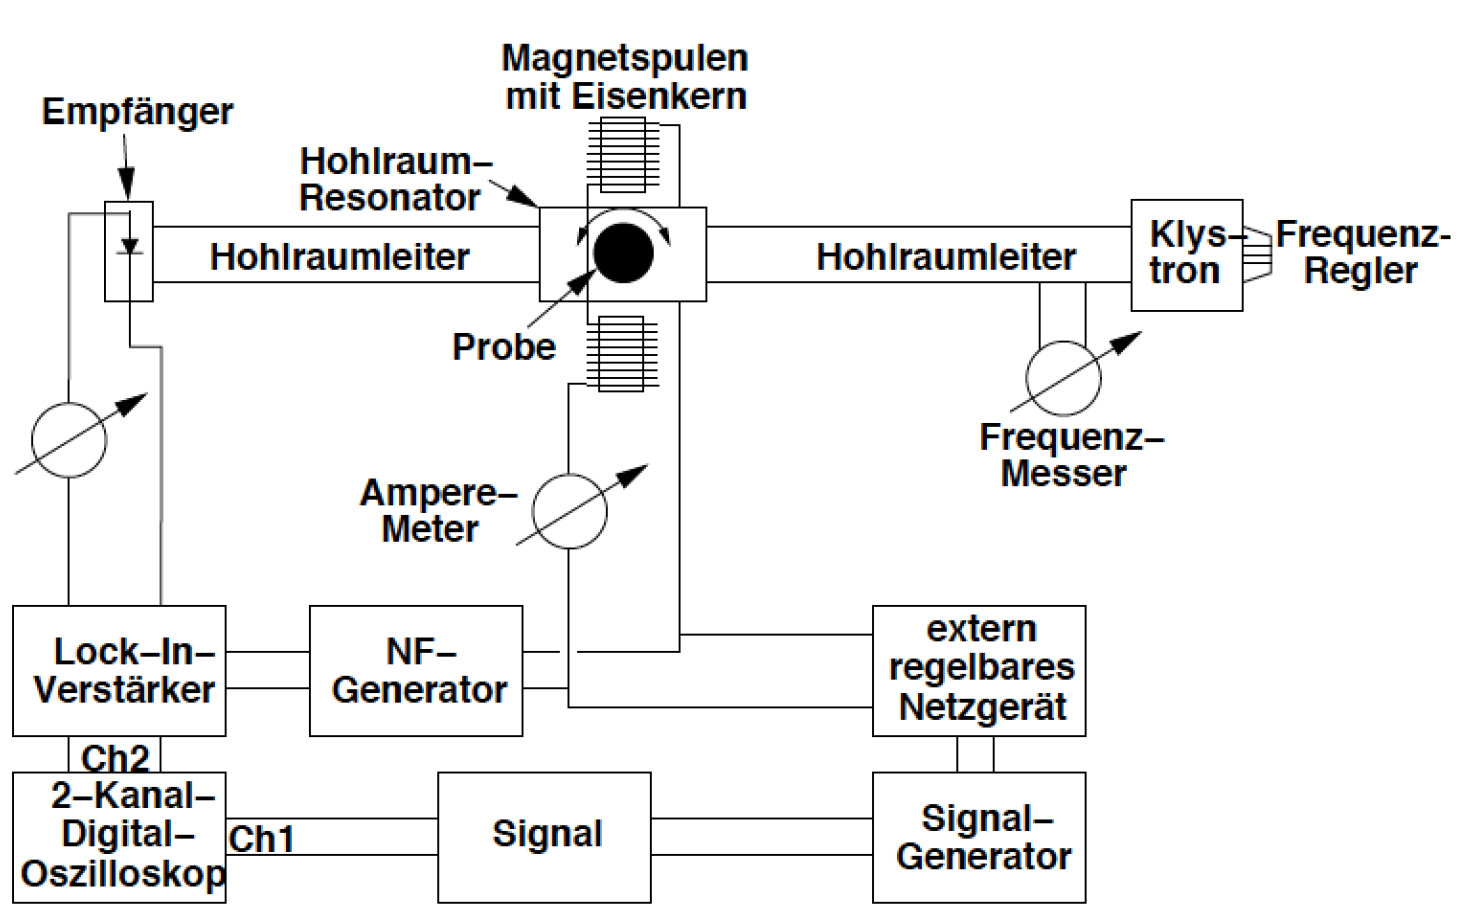
\includegraphics[scale=0.4]{Versuchsaufbau.png}
    \caption{Schematischer Versuchsaufbau zur Elektronenspinresonanz (Abbildung aus \cite{Anleitung}, S.5)}
    \label{fig:Aufbau}
\end{figure}

\subsubsection{Klystron}
Der schematische Aufbau eines Klystrons zur Erzeugung von Mikrowellen ist in Abbildung \ref{fig:Klystron} grafisch dargestellt.

\begin{figure}[h!]
    \centering
    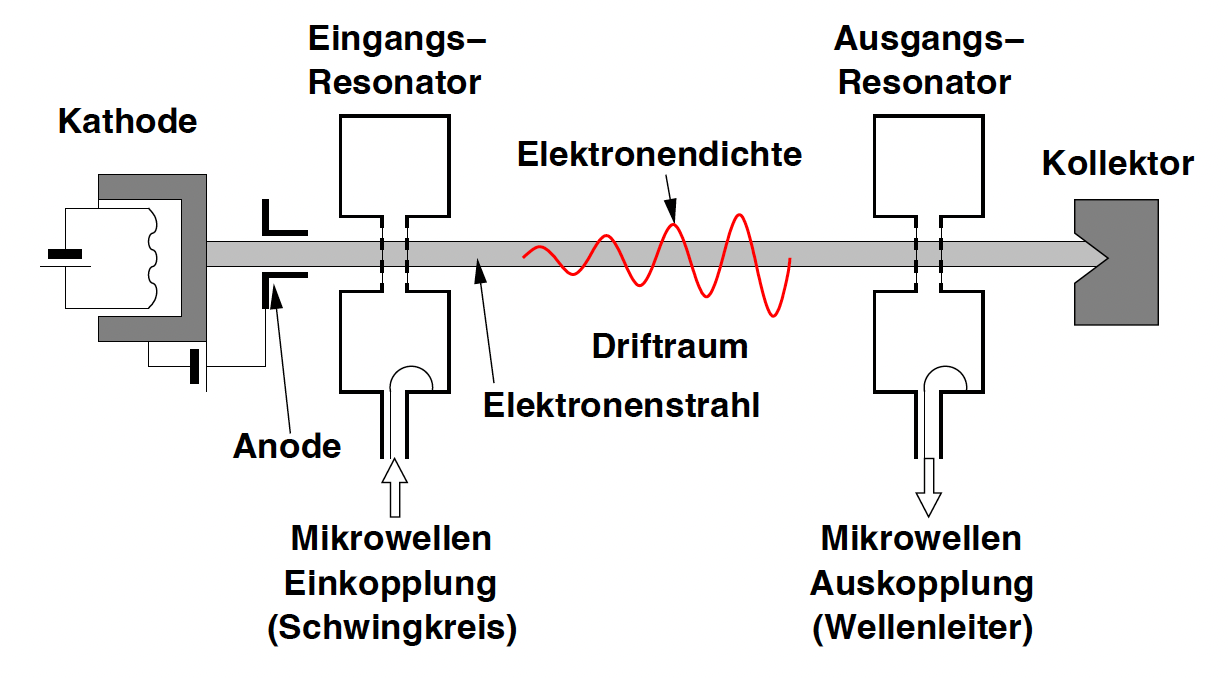
\includegraphics[scale=0.4]{Klystron.png}
    \caption{Schematischer Aufbau eines Zwei-Kammer Klystrons (Abbildung aus \cite{Grundlagen}, S. 19)}
    \label{fig:Klystron}
\end{figure}

Ein aus der Kathode austretender Elektronenstrahl wird mittels Hochspannung zum ersten Resonator hin beschleunigt. Dieser dient zunächst zur Einspeisung von Mikrowellen der gewünschten Frequenz, welche  durch einen Schwingkreis erzeugt werden. Je nach Phasenlage werden die Elektronen dementsprechend beschleunigt oder gebremst. Im anschließenden Driftraum bewegen sich die Elektronen mit ihrer individuellen Geschwindigkeit, sodass ein dichtemodulierter Strahl entsteht, wenn die schnelleren die langsameren Elektronen einholen. Im Ausgangsresonator induziert der Elektronenstrahl nun eine Wechselspannung, welche in Form eines Mikrowellen-Wechselfeldes ausgekoppelt und für den weiteren Versuchsaufbau verwendet wird. Der Energiegewinn im ausgekoppelten Feld folgt aus der kinetischen Energie des Elektronenstrahls. Im Versuch wird der Kollektor durch einen Reflektor ersetzt, welcher den Elektronenstrahl reflektiert, sodass das Klystron mit nur einem Resonator auskommt.


\subsubsection{Hohlraumleiter und -resonator}
Ein Hohlleiter dient zum Transport hochfrequenter elektromagnetischer Wellen. Seine Abmessungen entsprechen der Größenordnung der Wellenlänge der zu leitenden Strahlung, sodass nur bestimmte Frequenzen übertragen werden können. Dies geschieht dadurch, dass sich durch Reflexion an den Wänden des Leiters vertikal und horizontal stehende Wellen bilden, welche sich in z-Richtung ausbreiten. Im Versuch wird das im Klystron erzeugte Mikrowellenfeld in den Hohlleiter eingekoppelt und darin zur Probe geleitet. \\

Die Probe befindet sich innerhalb eines Hohraumresonators, welcher zur Verstärkung des Effekts der Spinresonanz benötigt wird. Im Inneren des Resonators werden Schwingungsmoden mit bestimmten Eigenfrequenzen angeregt, sodass sich eine stehende Welle bildet. Da sich die Eigenfrequenz des Resonators bei Rotation der Probe ändert, muss durch Anpassung am Klystron jeweils sichergestellt werden, dass die Frequenzen übereinstimmen.

\subsubsection{Hallsonde}

Um letztendlich den Landé-Faktor der Probe zu bestimmen, wird diese in ein äußeres Magnetfeld gebracht, welches langsam variiert werden kann. Die eingestrahlten Mikrowellen haben eine bekannte Frequenz, wodurch der Wert des Magnetfeldes ermittelt werden kann, bei welchem Resonanz auftritt, das heißt, die Mikrowellen durch die Probe absorbiert werden. Die Gleichung zur Berechnung des g-Faktors lautet dann:
\begin{equation}
    h \nu = g \mu_B B \, .
\end{equation} 

Zur Messung des Magnetfeldes wird eine Hall-Sonde verwendet. Der zugrundeliegende Effekt ist der Hall-Effekt in Halbleitern, welcher in Abbildung \ref{fig:Halleffekt} grafisch dargestellt ist. Er beschreibt die durch die Lorentz-Kraft bedingte Ablenkung von Ladungsträgern in einem Leiter, welcher in ein äußeres Magnetfeld gebracht wird. 

\begin{figure}[h!]
    \centering
    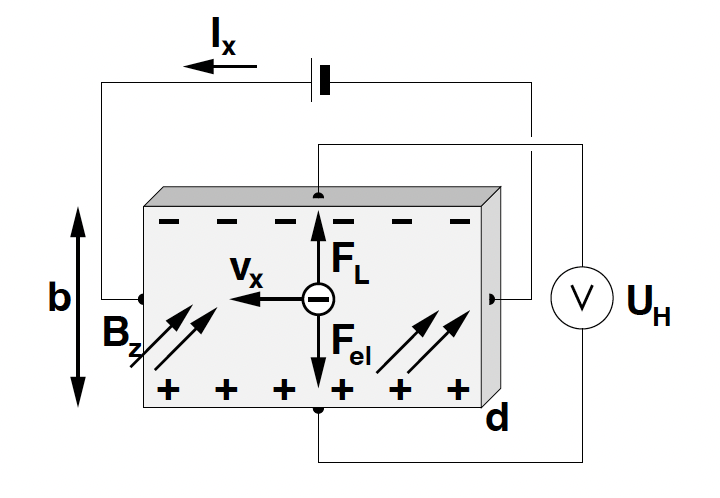
\includegraphics[scale=0.35]{Halleffekt.png}
    \caption{Hall-Effekt in einem Halbleiter (Abbildung aus \cite{Grundlagen}, S. 23)}
    \label{fig:Halleffekt}
\end{figure}

Die Hall-Sonde besteht aus einem Plättchen der Dicke \textit{d} und Breite \textit{b}, welches senkrecht zum Magnetfeld angebracht wird. Das Magnetfeld sorgt für eine Ladungstrennung innerhalb der Sonde. Die dadruch entstehende Spannung kann nun abgegriffen und gemessen werden und ist proportional zum angelegten Magnetfeld:
\begin{equation}
    U_H = R_H \frac{I_x \cdot B_z}{d}
\end{equation}
mit dem Strom $I_x$ durch den Halbleiter, der z-Komponente des Magnetfeldes $B_z$ und der Hall-Konstante $R_H$.

\subsubsection{Lock-in-Verstärker}
Das Ziel des Versuchs ist es, die durch die Absorption der Probe verursachte Änderung der Mikrowellenleistung zu bestimmen. Da diese sehr gering ist, muss sie zunächst mittels eines Lock-in-Verstärkers verstärkt werden. Zunächst wird die Amplitude des Signals mittels eines schwachen sinusförmigen Signals moduliert. Um das Messsignal aus dem Eingangssignal herauszufiltern, wird dieses mit einem Referenzssignal gleicher Frequenz multipliziert und dadurch gleichgerichtet. Ein anschließender Tiefpass-Filter glättet das Signal.



\section{Versuchsdurchführung und Auswertung}
Die Elektronenspinresonanz der beiden Proben CuSO4 und DPPH sollen in Abhängigkeit vom Winkel, mit der die Probe im Hohlraum-Resonator eingebaut werden, untersucht werden. Um zu bestimmen welche Magnetfeldstärke von den Proben absorbiert wird, wird die an den Spulen angelegte Spannung von \SI{1.5}{V} bis \SI{3}{V} variiert. Aus dem im Signal sichtbaren Peak kann das Magnetfeld bestimmt werden, bei dem die Elektronenspinresonanz auftritt. 

\subsection{Magnetfeldkalibration}
Um den gemessenen angelegten Spannungen ein Magnetfeld zuzuordnen, muss zunächst eine Magnetfeldkalibration durchgeführt werden.
Hierzu erzeugen wir mit einem Oszilloskop ein Signal mit einer konstanten Spannung von \SI{1.5}{V} bis \SI{3}{V} in \SI{0.1}{V} Abständen erzeugt. Da man mit dem Oszilloskop nur periodisch schwingende Signale erzeugen kann, stellen wir das Oszilloskop so ein, dass es eine sehr geringe Amplitude von \SI{4}{mV} hat und um den entsprechend eingestellten Offset hat. Da der Offset deutlich größer als die eingestellte Amplitude ist handelt es sich um ein annährend konstantes Signal. 
Das bei der eingestellten Spannung entstehende Magnetfeld messen wir mit einer Hall-Sonde, die in das Innere des Hohlraum-Resonators eingebaut wird. Wir messen für jede Spannungsstufe die Magnetfeldstärke bei ansteigender und abfallender Spannung. Dies ist notwendig, da bei abfallender Spannung bereits ein Magnetfeld anliegt. Dieses verlangsamt den Abbau des Magnetfelds bei Verringerung der Spannung, da das bestehende Feld einen Strom in der Spule induziert, der das Magnetfeld aufrechterhält. Der Verlauf der Spannung ist in Grafik \ref{fig:Spannung} dargestellt. 
\begin{figure}[h!]
    \centering
    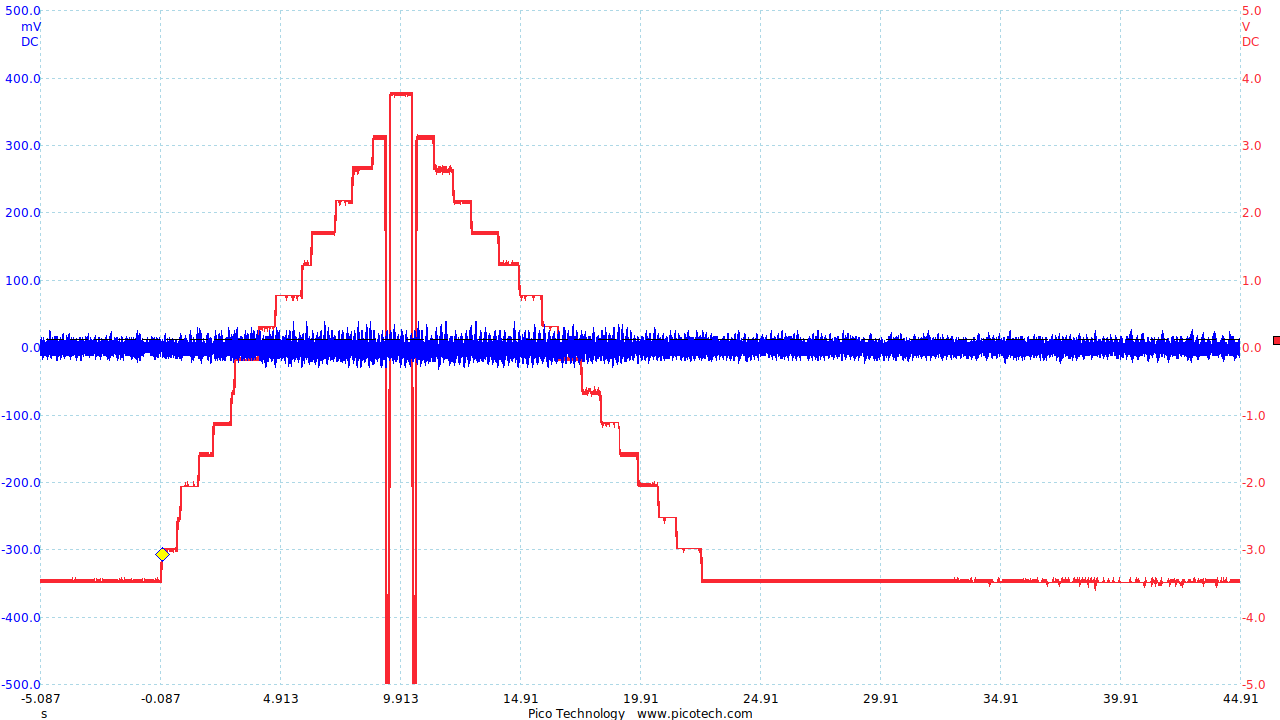
\includegraphics[scale=0.7]{3_1MagnetfeldkalibrationSpannungAufsteigundUndAbsteigend.png}
    \caption{Angelegte Spannungen für die Magnetfeldkalibration}
    \label{fig:Spannung}
\end{figure}
Die Kalibration muss ebenfalls durchgeführt werden, da die Spannungsversorgung erst aufgewärmt werden muss bevor eine Messung durchgeführt werden kann. 




\newpage
\section{Literaturverzeichnis}
\begin{thebibliography}{}
\bibitem{Fliesbach} Fließbach, T., 2018, \textit{Lehrbuch zur Theoretischen Physik III - Quantenmechanik}, 6. Auflage, Springer Spektrum, Berlin.
\bibitem{Demtroder} Demtröder, W., 2016, \textit{Experimentalphysik 3 - Atome, Moleküle und Festkörper}, 5. Auflage, Springer Spektrum, Berlin.
\bibitem{Grundlagen} \textit{Versuch Nr. 10 - Elektronenspinresonanz Grundlagen}, 2008
\bibitem{Anleitung} James, C.W., 2015, \textit{Experimental notes for the ESR Practical}

\end{thebibliography}

%\section{Anhang}
	
\end{document}
